\documentclass{article}

\usepackage{graphicx}
 
\begin{document}

\section{Instrumentation}

\begin{description}
        \item [Dumond diagram] Best geometry for 4-crystal monochromators
\end{description}

\begin{figure}
        \centering
        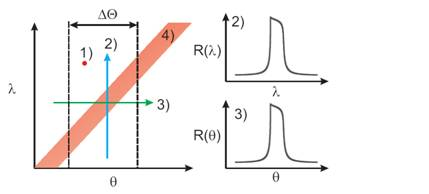
\includegraphics{dumonddiagram.jpg}
        \caption{DuMond diagram. Point 1) represents the planar electromagnetic wave, vertical line 2) represents the polychromatic parallel radiation and horizontal line represents the divergent monochromatic radiation. The crystal function in this space is represented as a stripe 4).}
\end{figure}



\end{document}

 
